% Created by tikzDevice version 0.12.3.1 on 2022-03-17 14:43:22
% !TEX encoding = UTF-8 Unicode
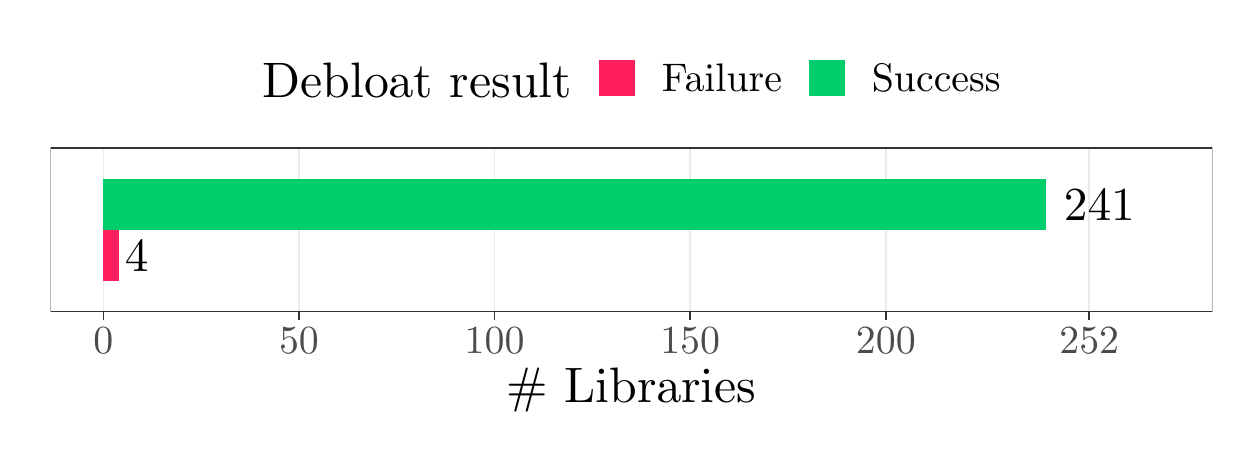
\begin{tikzpicture}[x=1pt,y=1pt]
\definecolor{fillColor}{RGB}{255,255,255}
\path[use as bounding box,fill=fillColor,fill opacity=0.00] (0,0) rectangle (433.62,144.54);
\begin{scope}
\path[clip] (  0.00,  0.00) rectangle (433.62,144.54);
\definecolor{drawColor}{RGB}{255,255,255}
\definecolor{fillColor}{RGB}{255,255,255}

\path[draw=drawColor,line width= 0.6pt,line join=round,line cap=round,fill=fillColor] (  0.00,  0.00) rectangle (433.62,144.54);
\end{scope}
\begin{scope}
\path[clip] (  8.25, 41.81) rectangle (428.12,101.14);
\definecolor{fillColor}{RGB}{255,255,255}

\path[fill=fillColor] (  8.25, 41.81) rectangle (428.12,101.14);
\definecolor{drawColor}{gray}{0.92}

\path[draw=drawColor,line width= 0.6pt,line join=round] ( 27.34, 41.81) --
	( 27.34,101.14);

\path[draw=drawColor,line width= 0.6pt,line join=round] ( 98.02, 41.81) --
	( 98.02,101.14);

\path[draw=drawColor,line width= 0.6pt,line join=round] (168.71, 41.81) --
	(168.71,101.14);

\path[draw=drawColor,line width= 0.6pt,line join=round] (239.39, 41.81) --
	(239.39,101.14);

\path[draw=drawColor,line width= 0.6pt,line join=round] (310.08, 41.81) --
	(310.08,101.14);

\path[draw=drawColor,line width= 0.6pt,line join=round] (383.59, 41.81) --
	(383.59,101.14);
\definecolor{fillColor}{RGB}{255,31,93}

\path[fill=fillColor] ( 27.34, 52.94) rectangle ( 32.99, 71.48);
\definecolor{fillColor}{RGB}{0,205,108}

\path[fill=fillColor] ( 27.34, 71.48) rectangle (368.04, 90.02);
\definecolor{drawColor}{RGB}{0,0,0}

\node[text=drawColor,anchor=base west,inner sep=0pt, outer sep=0pt, scale=  1.71] at ( 35.12, 56.33) {4};

\node[text=drawColor,anchor=base west,inner sep=0pt, outer sep=0pt, scale=  1.71] at (374.44, 74.87) {241};
\definecolor{drawColor}{gray}{0.20}

\path[draw=drawColor,line width= 0.6pt,line join=round,line cap=round] (  8.25, 41.81) rectangle (428.12,101.14);
\end{scope}
\begin{scope}
\path[clip] (  0.00,  0.00) rectangle (433.62,144.54);
\definecolor{drawColor}{gray}{0.20}

\path[draw=drawColor,line width= 0.6pt,line join=round] ( 27.34, 39.06) --
	( 27.34, 41.81);

\path[draw=drawColor,line width= 0.6pt,line join=round] ( 98.02, 39.06) --
	( 98.02, 41.81);

\path[draw=drawColor,line width= 0.6pt,line join=round] (168.71, 39.06) --
	(168.71, 41.81);

\path[draw=drawColor,line width= 0.6pt,line join=round] (239.39, 39.06) --
	(239.39, 41.81);

\path[draw=drawColor,line width= 0.6pt,line join=round] (310.08, 39.06) --
	(310.08, 41.81);

\path[draw=drawColor,line width= 0.6pt,line join=round] (383.59, 39.06) --
	(383.59, 41.81);
\end{scope}
\begin{scope}
\path[clip] (  0.00,  0.00) rectangle (433.62,144.54);
\definecolor{drawColor}{gray}{0.30}

\node[text=drawColor,anchor=base,inner sep=0pt, outer sep=0pt, scale=  1.44] at ( 27.34, 26.95) {0};

\node[text=drawColor,anchor=base,inner sep=0pt, outer sep=0pt, scale=  1.44] at ( 98.02, 26.95) {50};

\node[text=drawColor,anchor=base,inner sep=0pt, outer sep=0pt, scale=  1.44] at (168.71, 26.95) {100};

\node[text=drawColor,anchor=base,inner sep=0pt, outer sep=0pt, scale=  1.44] at (239.39, 26.95) {150};

\node[text=drawColor,anchor=base,inner sep=0pt, outer sep=0pt, scale=  1.44] at (310.08, 26.95) {200};

\node[text=drawColor,anchor=base,inner sep=0pt, outer sep=0pt, scale=  1.44] at (383.59, 26.95) {252};
\end{scope}
\begin{scope}
\path[clip] (  0.00,  0.00) rectangle (433.62,144.54);
\definecolor{drawColor}{RGB}{0,0,0}

\node[text=drawColor,anchor=base,inner sep=0pt, outer sep=0pt, scale=  1.80] at (218.18,  9.00) {\# Libraries};
\end{scope}
\begin{scope}
\path[clip] (  0.00,  0.00) rectangle (433.62,144.54);
\definecolor{fillColor}{RGB}{255,255,255}

\path[fill=fillColor] ( 79.31,112.14) rectangle (357.06,139.04);
\end{scope}
\begin{scope}
\path[clip] (  0.00,  0.00) rectangle (433.62,144.54);
\definecolor{drawColor}{RGB}{0,0,0}

\node[text=drawColor,anchor=base west,inner sep=0pt, outer sep=0pt, scale=  1.80] at ( 84.81,119.39) {Debloat result};
\end{scope}
\begin{scope}
\path[clip] (  0.00,  0.00) rectangle (433.62,144.54);
\definecolor{fillColor}{RGB}{255,255,255}

\path[fill=fillColor] (205.68,119.09) rectangle (220.13,133.54);
\end{scope}
\begin{scope}
\path[clip] (  0.00,  0.00) rectangle (433.62,144.54);
\definecolor{fillColor}{RGB}{255,31,93}

\path[fill=fillColor] (206.39,119.80) rectangle (219.42,132.83);
\end{scope}
\begin{scope}
\path[clip] (  0.00,  0.00) rectangle (433.62,144.54);
\definecolor{fillColor}{RGB}{255,255,255}

\path[fill=fillColor] (281.56,119.09) rectangle (296.02,133.54);
\end{scope}
\begin{scope}
\path[clip] (  0.00,  0.00) rectangle (433.62,144.54);
\definecolor{fillColor}{RGB}{0,205,108}

\path[fill=fillColor] (282.27,119.80) rectangle (295.30,132.83);
\end{scope}
\begin{scope}
\path[clip] (  0.00,  0.00) rectangle (433.62,144.54);
\definecolor{drawColor}{RGB}{0,0,0}

\node[text=drawColor,anchor=base west,inner sep=0pt, outer sep=0pt, scale=  1.44] at (229.13,121.35) {Failure};
\end{scope}
\begin{scope}
\path[clip] (  0.00,  0.00) rectangle (433.62,144.54);
\definecolor{drawColor}{RGB}{0,0,0}

\node[text=drawColor,anchor=base west,inner sep=0pt, outer sep=0pt, scale=  1.44] at (305.02,121.35) {Success};
\end{scope}
\end{tikzpicture}
